% !TEX program = xelatex

\documentclass{VUMIFPSkursinis}
\usepackage{algorithmicx}
\usepackage{algorithm}
\usepackage{algpseudocode}
\usepackage{amsfonts}
\usepackage{amsmath}
\usepackage{bm}
\usepackage{caption}
\usepackage{color}
\usepackage{float}
\usepackage{graphicx}
\usepackage{listings}
\usepackage{float}
\usepackage{subfig}
\usepackage{wrapfig}
\usepackage[hidelinks]{hyperref}
\usepackage{todonotes}
\usepackage{lineno}

% Titulinio aprašas
\university{Vilniaus universitetas}
\faculty{Matematikos ir informatikos fakultetas}
\department{}
\papertype{Programų sistemų inžinerijos modeliai ir metodai laboratorinis darbas 2}
\title{Requirements modeling}
\titleineng{Reikalavimų modeliavimas}
\status{1 course students}
\author{Matas Savickis}
\secondauthor{Vytautas Krivickas}
\thirdauthor{Šarūnas Kazimieras Buteikis}


\supervisor{Audronė Lupeikienė, M. Darbuot., Dr}
\date{Vilnius – \the\year}

% Nustatymai
% \setmainfont{Palemonas}   % Pakeisti teksto šriftą į Palemonas (turi būti įdiegtas sistemoje)
\bibliography{bibliografija}

\begin{document}
\selectlanguage{english}
\maketitle

\tableofcontents

\section{NFR type catalogue}

\begin{figure}[htbp]
	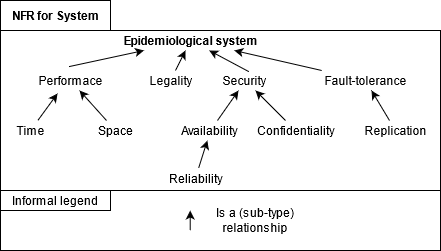
\includegraphics[scale=0.6]{img/1}
	\caption{NFR diagram} % Antraštė įterpiama po paveikslėlio
	\label{img:kurimoProcesas}
\end{figure}

	\begin{itemize}
		\item{Virus registration time}
		\item{Patient notification time}
		\item{Holding medical records}
		\item{Holding foreign countries data}
		\item{Reliability}
		\item{Distributivity}
		\item{Confidentiality}
		\item{Completness}
		\item{Minimality}
		\item{Summarizability}
		\item{Domain Compliance}
		\item{Tracebility}
		\item{LTU law}
		\item{GDPR}
		\item{Replication}
		\item{Tolerance algorithm}
	\end{itemize}

\section{Modelling of the non-functional requirements}

\section{Identifying and modelling of possible operationalizations for NFR}

\section{Detecting and modelling of implicit interdependencies among NFR}

\section{Chosen operationalizations}

\section{Strategic rationale model}

\section{Conclusions about an actor dependency}

\sectionnonum{Conclusions}

\end{document}
